% =====================================================================
% Báo cáo Seminar S04: LIME và SHAP (bản tiếng Việt)
% Biên dịch bằng XeLaTeX (Overleaf: Menu -> Compiler -> XeLaTeX)
% Hình nằm trong thư mục figs_en/ (nhãn trên hình là tiếng Anh)
%
% Đây là bản dịch của Report.tex. Mọi số liệu, bảng, công thức và kết
% luận giữ nguyên như bản tiếng Anh; chỉ phần diễn đạt được chuyển ngữ.
% =====================================================================
\documentclass[11pt,a4paper]{article}
\usepackage[a4paper,margin=2.0cm]{geometry}
\emergencystretch=2em
\usepackage{fontspec}
% TeX Gyre Termes: bản sao Times, đi kèm TeX Live nên biên dịch được cả trên
% Overleaf/Linux, và phủ đủ dấu tiếng Việt. Dùng font hệ thống "Times New Roman"
% thì copy-paste từ PDF sẽ bị mất dấu cách giữa các từ.
\setmainfont{TeX Gyre Termes}
\usepackage{amsmath,amssymb}
\usepackage{booktabs,tabularx,array}
\usepackage{graphicx}
\usepackage{float}
\usepackage[font=small,labelfont=bf]{caption}
\usepackage{enumitem}
\usepackage{pgfplots}
\pgfplotsset{compat=1.16}
\usepackage[colorlinks=true,linkcolor=black,urlcolor=blue,citecolor=black]{hyperref}

\setlist{itemsep=2pt,topsep=3pt,parsep=0pt}
\setlength{\parindent}{0pt}
\setlength{\parskip}{5pt}
\renewcommand{\arraystretch}{1.15}
\newcolumntype{L}[1]{>{\raggedright\arraybackslash}p{#1}}
\newcommand{\code}[1]{\texttt{#1}}
\newcommand{\coderepo}{\href{https://github.com/khoiLearnsToCode/CS420_AI_LIME_SHAP}{kho mã nguồn}}

\renewcommand{\abstractname}{Tóm tắt}
\renewcommand{\refname}{Tài liệu tham khảo}
\renewcommand{\figurename}{Hình}
\renewcommand{\tablename}{Bảng}
\renewcommand{\appendixname}{Phụ lục}
\renewcommand{\contentsname}{Mục lục}

\title{\textbf{LIME và SHAP: Giải thích dự đoán của mô hình học máy}\\[2pt]\large Báo cáo Seminar S04 -- CS420}
\author{%
  Nguyễn Trọng Hoàng\\ \small 24125056 \and
  Phan Minh Khôi\\ \small 24125061 \and
  Nguyễn Thuận Việt\\ \small 24125051%
}
\date{}

\begin{document}
\maketitle

\begin{abstract}
Các mô hình học máy ngày càng được dùng trong những lĩnh vực có rủi ro cao
như y khoa, nhưng một mô hình thường xuyên dự đoán đúng không vì thế mà tự
động cho biết \emph{vì sao} nó đưa ra một quyết định cụ thể. Báo cáo này đặt
câu hỏi: liệu một dự đoán có độ chính xác cao có nhất thiết đi kèm một lời
giải thích đáng tin cậy hay không. Chúng tôi tập trung vào hai công cụ được
dùng phổ biến là LIME (Local Interpretable Model-agnostic Explanations) và
SHAP (SHapley Additive exPlanations), vốn ước lượng mức đóng góp của từng
đặc trưng đầu vào vào một dự đoán đơn lẻ. Chúng tôi áp dụng cả hai công cụ
lên hai mô hình được huấn luyện để phát hiện ung thư vú từ các phép đo khối
u, rồi khảo sát ba trường hợp: một mẫu dễ, một mẫu sát ranh giới và một mẫu
bị dự đoán sai; với mỗi trường hợp, chúng tôi hỏi hai công cụ có đồng thuận
không, kết quả có giữ nguyên khi chạy lại không, và những đặc trưng được xếp
hạng cao có thực sự chi phối dự đoán không. Mặc dù hai mô hình đạt độ chính
xác 98,2\% và 95,6\%, hai công cụ chỉ đồng thuận tốt ở mẫu dễ: trên mẫu bị
dự đoán sai, chúng chỉ chia sẻ hai trong năm đặc trưng quan trọng nhất, và
thứ hạng thay đổi rõ rệt giữa các lần chạy. Cả hai đều tìm ra đặc trưng có
ảnh hưởng tốt hơn hẳn so với chọn ngẫu nhiên, nhưng không công cụ nào tỏ ra
đáng tin cậy hơn công cụ còn lại. Vì vậy, chúng tôi khuyến nghị lặp lại việc
giải thích và kiểm tra độ ổn định của nó trước khi tin tưởng, đặc biệt với
những dự đoán không chắc chắn hoặc sai.
\end{abstract}

%---------------------------------------------------------------------
\section{Giới thiệu}

Nhiều mô hình học máy hiện đại là những ``hộp đen'': ta thấy đầu vào và đầu
ra nhưng không biết đặc trưng nào chi phối quyết định. Trong y tế, tài chính
hay xe tự hành, một dự đoán không thể được tin tưởng chỉ vì nó thường đúng,
nên nhu cầu giải thích từng quyết định riêng lẻ ngày càng lớn
\cite{ribeiro}\cite{mersha}. LIME \cite{ribeiro} và SHAP \cite{lundberg} là
hai phương pháp post-hoc được dùng rộng rãi cho mục đích này.

\paragraph{Câu hỏi dẫn dắt.} Một dự đoán có độ chính xác cao có nhất thiết đi
kèm một lời giải thích đáng tin cậy hay không? Để trả lời, chúng tôi xét ba
tiêu chí: lời giải thích có \emph{hữu ích} hay không (nó cho thấy đặc trưng
nào đẩy dự đoán lên hoặc xuống), có \emph{ổn định} hay không (không thay đổi
theo seed hay theo dữ liệu nền) và có \emph{trung thực} với mô hình hay không
(xoá bỏ những đặc trưng được cho là quan trọng thì dự đoán phải thay đổi
tương ứng).

\paragraph{Phạm vi.} Chúng tôi dùng bộ dữ liệu Breast Cancer Wisconsin
\cite{street} (569 mẫu, 30 đặc trưng, hai lớp), hai mô hình (Logistic
Regression và Random Forest) và ba mẫu được chọn theo một quy tắc cố định.
Hai bài báo gốc là Ribeiro và cộng sự~\cite{ribeiro} cho LIME và Lundberg \&
Lee~\cite{lundberg} cho SHAP; bài khảo sát của Mersha và cộng
sự~\cite{mersha} được dùng để định vị cả hai phương pháp trong phân loại XAI
và để chọn tiêu chí đánh giá.

\paragraph{Đóng góp.} Chúng tôi (i) tổng hợp và so sánh hai bài báo bắt buộc
\cite{ribeiro}\cite{lundberg} cùng một bài khảo sát \cite{mersha}; (ii) tính
tay SHAP trên một mô hình tuyến tính và LIME trên một mô hình phi tuyến nhỏ;
(iii) so sánh hai phương pháp theo độ trùng top-$k$, thời gian chạy và độ ổn
định khi đổi seed cũng như đổi tập nền; và (iv) chạy một deletion test rồi đề
xuất một quy trình đánh giá độ trung thực. Những gì thuộc về các bài báo đều
có trích dẫn; phần ví dụ và số liệu còn lại là của nhóm.

%---------------------------------------------------------------------
\section{Cơ sở lý thuyết và tổng quan tài liệu}

\subsection{Các khái niệm cốt lõi}
Mersha và cộng sự~\cite{mersha} chỉ ra rằng thuật ngữ trong lĩnh vực XAI vẫn
chưa thống nhất. Trong báo cáo này, \emph{tính diễn giải được}
(interpretability) nghĩa là mức độ một người có thể hiểu được mô hình vận
hành bên trong ra sao, còn \emph{tính giải thích được} (explainability) là
khả năng đưa ra lý do cho \emph{một quyết định cụ thể}. Một số tác giả coi
khái niệm này là tập con của khái niệm kia, nên chúng tôi nêu rõ định nghĩa
của mình. Bảng~\ref{tab:concepts} liệt kê các cặp khái niệm được dùng trong
phần còn lại của báo cáo và cho thấy LIME cùng SHAP nằm ở đâu.

\begin{table}[!htb]
\centering\small
\caption{Các cặp khái niệm cốt lõi và vị trí của LIME, SHAP.}\label{tab:concepts}
\begin{tabularx}{\textwidth}{L{3.3cm}XX}
\toprule
\textbf{Cặp khái niệm} & \textbf{Phân biệt} & \textbf{LIME và SHAP}\\
\midrule
Giải thích được -- diễn giải được & Giải thích một dự đoán so với hiểu cách mô hình vận hành nói chung & Cung cấp tính giải thích được; không làm cho mô hình trở nên diễn giải được\\
Cục bộ -- toàn cục & Giải thích một mẫu so với mô tả toàn bộ mô hình & Cả hai đều cục bộ; LIME bổ sung SP-LIME để chọn các mẫu đại diện cho góc nhìn toàn cục \cite{ribeiro}\\
Phụ thuộc mô hình -- độc lập mô hình & Phụ thuộc cấu trúc mô hình so với chỉ cần hàm dự đoán & LIME và KernelSHAP độc lập mô hình; Linear SHAP và Deep SHAP phụ thuộc mô hình \cite{lundberg}\\
Nội tại (ante-hoc) -- post-hoc & Mô hình dễ hiểu ngay từ thiết kế so với được giải thích sau khi huấn luyện & Cả hai đều là post-hoc và dựa trên gây nhiễu \cite{mersha}\\
\bottomrule
\end{tabularx}
\end{table}

\subsection{LIME}\label{sec:lime}
LIME, do Ribeiro và cộng sự~\cite{ribeiro} đề xuất, giải thích một dự đoán
đơn lẻ bằng cách khớp một mô hình đơn giản bắt chước hộp đen trong vùng lân
cận của mẫu đang xét. Phương pháp lấy mẫu các điểm nhiễu quanh đầu vào $x$,
truy vấn mô hình hộp đen tại từng điểm, rồi khớp một mô hình thay thế dễ diễn
giải trong đó các điểm gần $x$ có trọng số lớn hơn. Về mặt hình thức, lời
giải thích là
\begin{equation}\label{eq:lime}
\xi(x) = \arg\min_{g \in G} \; L(f, g, \pi_x) + \Omega(g),
\end{equation}
\begin{equation}\label{eq:limeloss}
L(f, g, \pi_x) = \sum_{z, z'} \pi_x(z) \big( f(z) - g(z') \big)^2, \qquad \pi_x(z) = \exp\!\big( -D(x, z)^2 / \sigma^2 \big).
\end{equation}
Ở đây $f$ là mô hình hộp đen; trong các thực nghiệm của chúng tôi
$f(x) \in [0,1]$ là xác suất dự đoán của một lớp. $x \in \mathbb{R}^d$ là mẫu
cần giải thích ($d = 30$ với dữ liệu của chúng tôi), $z \in \mathbb{R}^d$ là
một mẫu nhiễu trong không gian đặc trưng gốc, và $z' \in \{0,1\}^N$ là biểu
diễn dễ diễn giải của nó trên $N$ thành phần diễn giải được, trong đó
$z'_i = 1$ nếu thành phần thứ $i$ có mặt trong $z$ và $z'_i = 0$ nếu không.
$G$ là họ các mô hình diễn giải được (ở đây là mô hình tuyến tính
$g(z') = w_g \cdot z'$), $D \geq 0$ là hàm khoảng cách (Euclid trong ví dụ
tính tay của chúng tôi) và $\sigma > 0$ là độ rộng kernel, nên
$\pi_x(z) \in (0, 1]$ và $L \geq 0$ được đo bằng đơn vị bình phương xác suất.
$\xi(x)$ là mô hình thay thế được chọn, và các trọng số $w_g$ của nó chính là
lời giải thích.

Hai thành phần trong Công thức~\eqref{eq:lime} định hình lời giải thích:
\begin{itemize}
  \item Kernel lân cận $\pi_x(z)$ xác định thế nào là ``cục bộ'': mẫu nhiễu
        càng gần $x$ thì trọng số càng lớn. Độ rộng kernel $\sigma$ quy định
        kích thước vùng lân cận này. Nếu $\sigma$ quá nhỏ, chỉ vài mẫu mang
        trọng số đáng kể và lời giải thích trở nên nhiễu; nếu quá lớn, mô
        hình thay thế không còn mang tính cục bộ.
  \item Thành phần phạt độ phức tạp $\Omega(g)$ giữ cho lời giải thích ngắn
        gọn. Với mô hình thay thế tuyến tính, Ribeiro và cộng sự đặt
        $\Omega(g) = \infty \cdot \mathbb{1}\big[\lVert w_g \rVert_0 > K\big]$,
        tức cấm có quá $K$ trọng số khác không, và dùng K-LASSO để chọn ra
        $K$ đặc trưng được giữ lại. Điều này đánh đổi một phần độ khớp cục bộ
        để lấy tính dễ đọc.
\end{itemize}

\subsection{SHAP}
\label{sec:shap}
SHAP, do Lundberg và Lee~\cite{lundberg} giới thiệu, xuất phát từ một lớp
phương pháp mà các tác giả gọi là \emph{quy gán đóng góp đặc trưng theo kiểu
cộng tính} (additive feature attribution). Trong lớp này, mô hình giải thích
là một hàm tuyến tính của các biến nhị phân:
\begin{equation}
g(z') = \varphi_0 + \sum_{j=1}^{M} \varphi_j z'_j, \qquad z' \in \{0, 1\}^M,
\end{equation}
trong đó $\varphi_j$ là phần đóng góp được quy cho đặc trưng $j$ và $M$ là số
đặc trưng ($M = 30$ với dữ liệu của chúng tôi). Các giá trị quy gán có cùng
đơn vị với $f$: trong thực nghiệm của chúng tôi $\varphi_0 \in [0, 1]$ và mỗi
$\varphi_j \in [-1, 1]$ là một mức thay đổi xác suất. Các tác giả chứng minh
(Định lý~1) rằng chỉ có duy nhất một cách quy gán trong lớp này thoả mãn đồng
thời ba tính chất:
\begin{itemize}
  \item \emph{độ chính xác cục bộ} (local accuracy): lời giải thích tái tạo
        lại đúng dự đoán, $g(x') = f(x)$;
  \item \emph{tính khuyết} (missingness): đặc trưng vắng mặt không nhận phần
        đóng góp nào;
  \item \emph{tính nhất quán} (consistency): nếu mô hình thay đổi sao cho
        đóng góp biên của một đặc trưng không giảm, thì phần quy gán cho nó
        cũng không giảm.
\end{itemize}
Nghiệm duy nhất này chính là giá trị Shapley:
\begin{equation}
\varphi_j = \sum_{S \subseteq F \setminus \{j\}} \frac{|S|! \, (M - |S| - 1)!}{M!} \Big[ f_{S \cup \{j\}}(x_{S \cup \{j\}}) - f_S(x_S) \Big].
\end{equation}
Ở đây $F$ là tập toàn bộ $M$ đặc trưng, $S$ là một tập con không chứa đặc
trưng $j$, và $f_S$ là dự đoán khi chỉ biết các đặc trưng trong $S$; những
đặc trưng còn lại được lấy trung bình trên một tập dữ liệu nền. Có ba đại
lượng cần nắm khi đọc một lời giải thích SHAP:
\begin{itemize}
  \item \textbf{Giá trị nền.} $\varphi_0 = \mathbb{E}[f(X)]$ là dự đoán trung
        bình trên dữ liệu nền, nên nó phụ thuộc vào cách chọn tập dữ liệu đó.
  \item \textbf{Phần đóng góp.} $\varphi_j$ là phần của khoảng cách giữa
        $f(x)$ và giá trị nền mà đặc trưng $j$ chịu trách nhiệm; cộng lại,
        $\varphi_0 + \sum_j \varphi_j = f(x)$ một cách chính xác.
  \item \textbf{Dấu.} $\varphi_j$ dương đẩy dự đoán lên trên giá trị nền,
        $\varphi_j$ âm kéo xuống dưới.
\end{itemize}
KernelSHAP ước lượng các giá trị Shapley bằng hồi quy tuyến tính có trọng số.
Lundberg và Lee chỉ ra rằng đây chính là LIME với một lựa chọn cụ thể về
kernel, hàm mất mát và thành phần điều chuẩn (Định lý~2), đồng thời lưu ý
rằng những lựa chọn mang tính heuristic của LIME cho các thành phần này có
thể vi phạm độ chính xác cục bộ hoặc tính nhất quán. Việc ước lượng thường
giả định các đặc trưng độc lập với nhau, và một số biến thể còn giả định mô
hình là tuyến tính. Với mô hình tuyến tính và các đặc trưng độc lập, giá trị
Shapley có dạng đóng $\varphi_j = w_j (x_j - \mathbb{E}[X_j])$, và đây là cơ
sở cho ví dụ tính tay ở Mục~\ref{sec:shaphand}.

\subsection{Bài khảo sát của Mersha và cộng sự}
Mersha và cộng sự~\cite{mersha} phân loại các kỹ thuật XAI theo bốn trục:
phạm vi (cục bộ hay toàn cục), giai đoạn (ante-hoc hay post-hoc), khả năng áp
dụng (phụ thuộc mô hình hay độc lập mô hình) và phương pháp luận thiết kế
(dựa trên gây nhiễu hay dựa trên gradient). Để đánh giá lời giải thích, các
tác giả tách riêng hướng lấy con người làm trung tâm và hướng lấy máy tính
làm trung tâm, rồi liệt kê năm tiêu chí thuộc hướng thứ hai: độ trung thực
(fidelity), tính nhất quán (consistency), tính bền vững (robustness), hiệu
quả (efficiency) và tính đầy đủ (sufficiency). Các tác giả cũng nhấn mạnh
rằng không có một thước đo duy nhất phù hợp cho mọi hệ thống. Chúng tôi dùng
các tiêu chí này để tổ chức phần đánh giá ở Mục~\ref{sec:results}.

\subsection{So sánh ba nguồn tài liệu}
Bảng~\ref{tab:sources} so sánh mục tiêu, đóng góp chính và hạn chế của ba
nguồn tài liệu.

\begin{table}[!htb]
\centering\small
\caption{So sánh ba nguồn tài liệu chính.}\label{tab:sources}
\begin{tabularx}{\textwidth}{L{3.0cm}XXX}
\toprule
\textbf{Nguồn} & \textbf{Mục tiêu} & \textbf{Đóng góp chính} & \textbf{Hạn chế / ghi chú}\\
\midrule
Ribeiro và cộng sự~\cite{ribeiro} & Giải thích dự đoán của bất kỳ bộ phân lớp nào để người dùng quyết định có nên tin hay không & LIME (mô hình thay thế thưa, có trọng số cục bộ) và SP-LIME để chọn mẫu đại diện & Kernel và $\sigma$ được chọn theo heuristic; không có bảo đảm kiểu Shapley\\
Lundberg \& Lee~\cite{lundberg} & Thống nhất các phương pháp quy gán đóng góp đặc trưng đang có & Lớp quy gán cộng tính, nghiệm duy nhất của nó (giá trị Shapley) và KernelSHAP & Việc ước lượng giả định các đặc trưng độc lập; kết quả phụ thuộc dữ liệu nền\\
Mersha và cộng sự~\cite{mersha} & Khảo sát XAI: phân loại, ứng dụng và đánh giá & Hệ phân loại bốn trục và năm tiêu chí đánh giá & Chỉ đề cập LIME và SHAP một cách ngắn gọn; chúng tôi dùng tiêu chí của bài theo tinh thần, không dùng công thức chính xác của bài (Mục~\ref{sec:proc})\\
\bottomrule
\end{tabularx}
\end{table}

%---------------------------------------------------------------------
\section{Phương pháp và ví dụ tính tay}
Chúng tôi trình bày thiết lập thực nghiệm, sau đó tính tay một ví dụ nhỏ cho
mỗi phương pháp để người đọc có thể theo dõi được các phép tính đứng sau
Mục~\ref{sec:results}.

\subsection{Thiết lập thực nghiệm}
Chúng tôi dùng dữ liệu Breast Cancer Wisconsin \cite{street} từ scikit-learn
(lớp 0 = ác tính), chia phân tầng 80/20 (455 mẫu huấn luyện, 114 mẫu kiểm
thử), một mô hình Logistic Regression (LR) có chuẩn hoá và một Random Forest
(RF) 200 cây, với độ chính xác trên tập kiểm thử lần lượt là 98,2\% và
95,6\%. Cả hai phương pháp đều giải thích $P(\text{ác tính})$: SHAP dùng
KernelSHAP (100 mẫu nền, 2000 liên minh), LIME dùng cấu hình mặc định của thư
viện (5000 mẫu nhiễu, độ rộng kernel $\approx 4{,}11$). Mọi lựa chọn đều được
cố định trước khi nhìn vào kết quả và tất cả seed đều được ấn định;
Phụ lục~\ref{app:setup} trình bày thiết lập đầy đủ cùng lý do cho từng lựa
chọn.

\textbf{Đặc trưng.} 30 đặc trưng được tính từ ảnh số hoá của một mẫu chọc hút
kim nhỏ: mười phép đo nhân tế bào (bán kính, kết cấu, chu vi, diện tích, độ
mịn, độ chặt, độ lõm, số điểm lõm, tính đối xứng, chiều fractal), mỗi phép đo
được cho dưới ba dạng là giá trị trung bình, sai số chuẩn (``error'') và
trung bình của ba giá trị lớn nhất (``worst''). Mọi giá trị đều không âm và
dữ liệu không ghi đơn vị vật lý: các đặc trưng kích thước nằm trên thang đo
của ảnh (diện tích theo đơn vị bình phương của bán kính), còn lại là các tỉ
số không thứ nguyên hoặc thống kê mức xám. Khoảng giá trị của chúng chênh
lệch rất lớn, chẳng hạn mean radius $6{,}98$--$28{,}11$, worst area
$185$--$4254$ và mean smoothness $0{,}053$--$0{,}163$, đó là lý do LR dùng
đầu vào đã chuẩn hoá. Tên đặc trưng được giữ nguyên tiếng Anh để khớp với tên
cột trong dữ liệu, với mã nguồn và với nhãn trên các hình.

\textbf{Các mẫu được chọn.} Một quy tắc cố định áp dụng trên RF chọn ra ba
mẫu kiểm thử (Bảng~\ref{tab:instances}): dự đoán đúng với độ tin cậy cao
nhất, dự đoán có $|P - 0{,}5|$ nhỏ nhất, và mẫu bị dự đoán sai đầu tiên. Cách
làm này ngăn chúng tôi chọn những ví dụ có lợi cho mình.

\begin{table}[!htb]
\centering\small
\caption{Ba mẫu được chọn. $P > 0{,}5$ nghĩa là mô hình dự đoán ác tính.}\label{tab:instances}
\begin{tabular}{lccc}
\toprule
\textbf{Mẫu} & \textbf{Chỉ số test} & \textbf{Nhãn thật} & \textbf{$P$(ác tính), RF / LR}\\
\midrule
Đúng chắc chắn & 0 & ác tính & 1,000 / 1,000\\
Sát ranh giới & 16 & lành tính & 0,495 / 0,634 (LR sai)\\
Dự đoán sai & 3 & lành tính & 0,745 (RF sai) / 0,466\\
\bottomrule
\end{tabular}
\end{table}

\subsection{Ví dụ tính tay 1: SHAP trên mô hình tuyến tính}\label{sec:shaphand}
Trước khi áp dụng SHAP lên dữ liệu thật, chúng tôi tính tay trên một mô hình
tuyến tính nhỏ để cho thấy giá trị nền và các phần đóng góp được tính ra sao,
đồng thời kiểm tra chúng cộng lại đúng bằng dự đoán (độ chính xác cục bộ,
Mục~\ref{sec:shap}).
Giả sử mô hình $f(x) = b + \sum_j w_j x_j$, các đặc trưng độc lập, và dữ liệu
nền là giá trị trung bình $\mu_j = \mathbb{E}[X_j]$. Khi đó $\varphi_0 = f(\mu)$
và $\varphi_j = w_j (x_j - \mu_j)$. Lấy $b = 1$, $w = (2, -1, 0{,}5)$,
$\mu = (1, 2, 4)$ và mẫu $x = (3, 1, 6)$.
\begin{itemize}
  \item Giá trị nền: $\varphi_0 = f(\mu) = 1 + 2\cdot 1 - 1\cdot 2 + 0{,}5\cdot 4 = 3$.
  \item Dự đoán: $f(x) = 1 + 2\cdot 3 - 1\cdot 1 + 0{,}5\cdot 6 = 9$.
  \item Phần đóng góp: $\varphi_1 = 2(3 - 1) = 4$; $\varphi_2 = (-1)(1 - 2) = 1$; $\varphi_3 = 0{,}5(6 - 4) = 1$.
  \item Kiểm tra: $\varphi_0 + \varphi_1 + \varphi_2 + \varphi_3 = 3 + 4 + 1 + 1 = 9 = f(x)$.
\end{itemize}
Liệt kê toàn bộ các tập con bằng công thức Shapley gốc (với $v(S) = f$ trong
đó các đặc trưng thuộc $S$ nhận giá trị từ $x$ còn lại nhận giá trị trung
bình) cho ra cùng kết quả $(4, 1, 1)$. Đặc trưng 2 có $w_2 < 0$ nhưng
$x_2 < \mu_2$, nên phần đóng góp của nó vẫn dương: dấu của $\varphi_j$ phụ
thuộc cả vào hệ số lẫn vị trí của mẫu so với dữ liệu nền.

\subsection{Ví dụ tính tay 2: LIME từng bước}\label{sec:limehand}
Tiếp theo, chúng tôi chạy tay LIME trên một mô hình phi tuyến nhỏ để minh hoạ
ba bước của nó (gây nhiễu đầu vào, gán trọng số theo khoảng cách, và khớp một
mô hình tuyến tính có trọng số) và để so sánh các hệ số thu được với độ dốc
cục bộ thật của mô hình.

\paragraph{Mô hình và mẫu.} Chúng tôi dùng mô hình
\begin{equation}
f(x) = \operatorname{sigmoid}(x_1^2 - x_2), \qquad
\operatorname{sigmoid}(t) = \frac{1}{1 + e^{-t}}.
\end{equation}
Hàm sigmoid ánh xạ một số thực $t$ bất kỳ về một giá trị trong khoảng 0 và 1,
nên $f(x)$ có thể đọc như một xác suất, giống trong hồi quy logistic. Mô hình
này phi tuyến theo đầu vào, vừa vì hàm sigmoid vừa vì số hạng $x_1^2$, nên
một mô hình thay thế tuyến tính chỉ có thể xấp xỉ nó một cách cục bộ. Mẫu cần
giải thích là $x_0 = (1, 2)$, với
$f(x_0) = \operatorname{sigmoid}(1 - 2) = \operatorname{sigmoid}(-1) = 0{,}2689$.

Để ví dụ dễ theo dõi, chúng tôi đơn giản hoá ba điểm: dùng 6 điểm nhiễu cố
định thay vì lấy mẫu ngẫu nhiên, đặt độ rộng kernel $\sigma = 1$, và bỏ thành
phần phạt $\Omega$. Chúng tôi cũng dùng chính các đặc trưng gốc (đã dịch theo
$x_0$) làm biểu diễn diễn giải được thay cho vectơ nhị phân $z'$ ở
Mục~\ref{sec:lime}, để các hệ số có thể so sánh trực tiếp với độ dốc của $f$.

\paragraph{Bước 1: gây nhiễu và truy vấn.} Với mỗi điểm nhiễu $z$, tính đầu
ra của mô hình $f(z)$. Ví dụ, với $z = (1{,}3,\, 2{,}2)$ ta được
$f(z) = \operatorname{sigmoid}(z_1^2 - z_2) = \operatorname{sigmoid}(-0{,}51) = 0{,}3752$.

\paragraph{Bước 2: gán trọng số theo khoảng cách.} Tính khoảng cách
$D = \lVert z - x_0 \rVert$ và trọng số $\pi = \exp(-D^2/\sigma^2)$. Với
$z = (1{,}3,\, 2{,}2)$, $D = \sqrt{(1{,}3 - 1)^2 + (2{,}2 - 2)^2} = 0{,}361$
và $\pi = 0{,}878$. Điểm càng gần $x_0$ thì trọng số càng gần 1.
Bảng~\ref{tab:limepoints} liệt kê cả sáu điểm.

\begin{table}[!htb]
\centering\small
\caption{Sáu điểm nhiễu cố định trong ví dụ LIME.}\label{tab:limepoints}
\begin{tabular}{ccccc}
\toprule
$z_1$ & $z_2$ & $f(z)$ & $D$ & $\pi$\\
\midrule
1,3 & 2,2 & 0,3752 & 0,361 & 0,878\\
0,6 & 2,1 & 0,1493 & 0,412 & 0,844\\
1,2 & 1,5 & 0,4850 & 0,539 & 0,748\\
0,9 & 1,7 & 0,2911 & 0,316 & 0,905\\
1,5 & 2,4 & 0,4626 & 0,640 & 0,664\\
0,7 & 2,5 & 0,1182 & 0,583 & 0,712\\
\bottomrule
\end{tabular}
\end{table}

\paragraph{Bước 3: khớp mô hình tuyến tính có trọng số.} Khớp
$g(z) = \beta_0 + g_1 (z_1 - 1) + g_2 (z_2 - 2)$ bằng bình phương tối thiểu
có trọng số:
\begin{equation}
\beta = (A^\top W A)^{-1} A^\top W y,
\end{equation}
trong đó mỗi hàng của $A$ là $[1,\; z_1 - 1,\; z_2 - 2]$,
$W = \operatorname{diag}(\pi)$ chứa các trọng số và $y$ chứa sáu giá trị
$f(z)$. Hai hệ số $g_1$ và $g_2$ chính là lời giải thích của LIME: dự đoán
thay đổi bao nhiêu trên mỗi đơn vị thay đổi của từng đặc trưng quanh $x_0$.

\paragraph{Kết quả.} Với $\sigma = 1$, LIME cho $g_1 = 0{,}395$ và
$g_2 = -0{,}149$. Độ dốc thật của $f$ tại $x_0$ là
\begin{equation}
\frac{\partial f}{\partial x_1} = f(1-f)\cdot 2x_1 = 0{,}393, \qquad
\frac{\partial f}{\partial x_2} = -f(1-f) = -0{,}197,
\end{equation}
dùng đẳng thức $\operatorname{sigmoid}'(t) = \operatorname{sigmoid}(t)\,\big(1 - \operatorname{sigmoid}(t)\big)$.
Ước lượng $g_1$ gần như chính xác. Ước lượng $g_2$ đúng dấu nhưng lệch khoảng
0,05, vì chỉ dùng 6 điểm và $f$ bị cong trong vùng lân cận. Điều này cho thấy
ở quy mô nhỏ rằng một lời giải thích của LIME phụ thuộc vào tập mẫu nhiễu.
Đổi độ rộng kernel sang $\sigma = 0{,}3$ cho
$(g_1, g_2) = (0{,}362,\, -0{,}132)$, còn $\sigma = 3$ cho
$(0{,}397,\, -0{,}150)$. Trong ví dụ rất nhỏ này $\sigma$ ảnh hưởng không
đáng kể; Mục~\ref{sec:results} sẽ đo tác động của nó trên dữ liệu 30 chiều.

%---------------------------------------------------------------------
\section{Kết quả và thảo luận}\label{sec:results}

\subsection{Biểu đồ đóng góp đặc trưng}
\label{sec:charts}
Hình~\ref{fig:rf} (Random Forest) và Hình~\ref{fig:lr} (Logistic Regression)
cho thấy phần đóng góp của 8 đặc trưng lớn nhất. Màu cam đẩy
$P$(ác tính) lên, màu xanh kéo xuống. Với SHAP,
$\varphi_0 + \sum_j \varphi_j$ bằng đúng $f(x)$ trong cả sáu trường hợp (ví
dụ Random Forest, mẫu 0: $0{,}326 + 0{,}674 = 1{,}000$), đúng như độ chính
xác cục bộ đòi hỏi.
\begin{itemize}
  \item \textbf{Mẫu đúng chắc chắn (RF):} cả LIME và SHAP đều xếp các đặc
        trưng về kích thước khối u (worst area, worst perimeter, worst
        radius, worst concave points) lên đầu, tất cả đều đẩy về phía ác
        tính.
  \item \textbf{Mẫu sát ranh giới (RF, $P = 0{,}495$):} các phần đóng góp đều
        nhỏ và lẫn lộn về dấu; LIME xếp worst concavity, mean texture và
        worst texture lên đầu, trong khi SHAP xếp worst perimeter, mean
        concave points (âm) và worst concavity lên đầu.
  \item \textbf{Mẫu bị dự đoán sai (RF, $P = 0{,}745$):} xem
        Mục~\ref{sec:wrong}.
\end{itemize}

\begin{figure}[!htb]
\centering
\begin{minipage}[t]{0.495\textwidth}
\centering
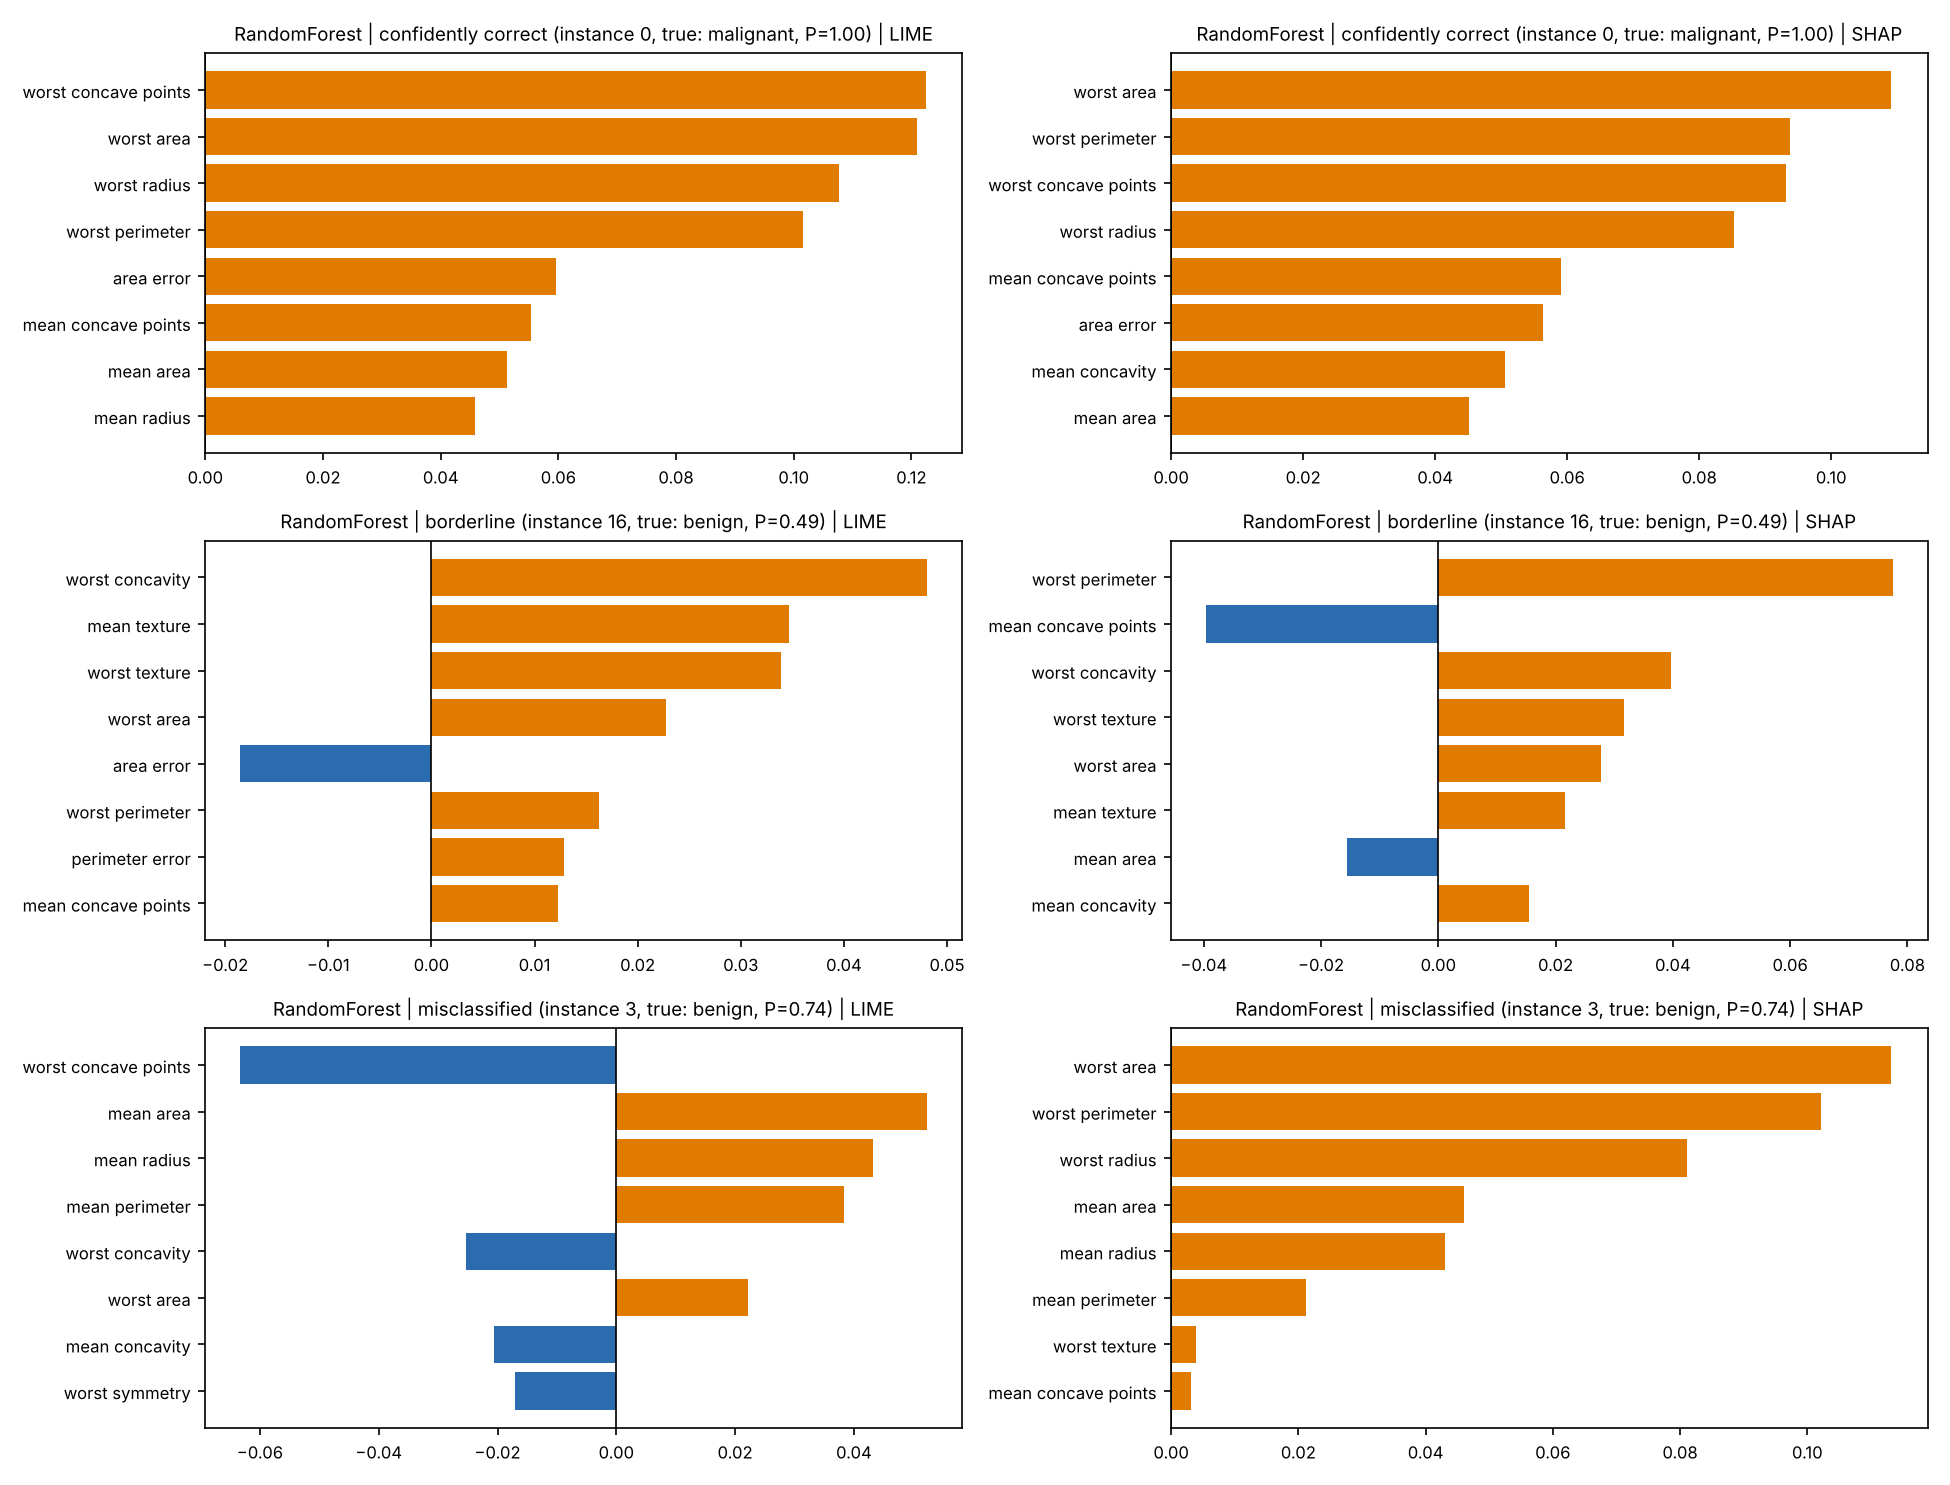
\includegraphics[width=\linewidth]{figs_en/contrib_RandomForest.png}
\caption{Phần đóng góp đặc trưng từ LIME (cột trái) và SHAP (cột phải) cho Random Forest; ba mẫu, từ trên xuống, là đúng chắc chắn, sát ranh giới và dự đoán sai. Nhãn trên hình là tiếng Anh. Nguồn: thực nghiệm của nhóm (\coderepo).}\label{fig:rf}
\end{minipage}\hfill
\begin{minipage}[t]{0.495\textwidth}
\centering
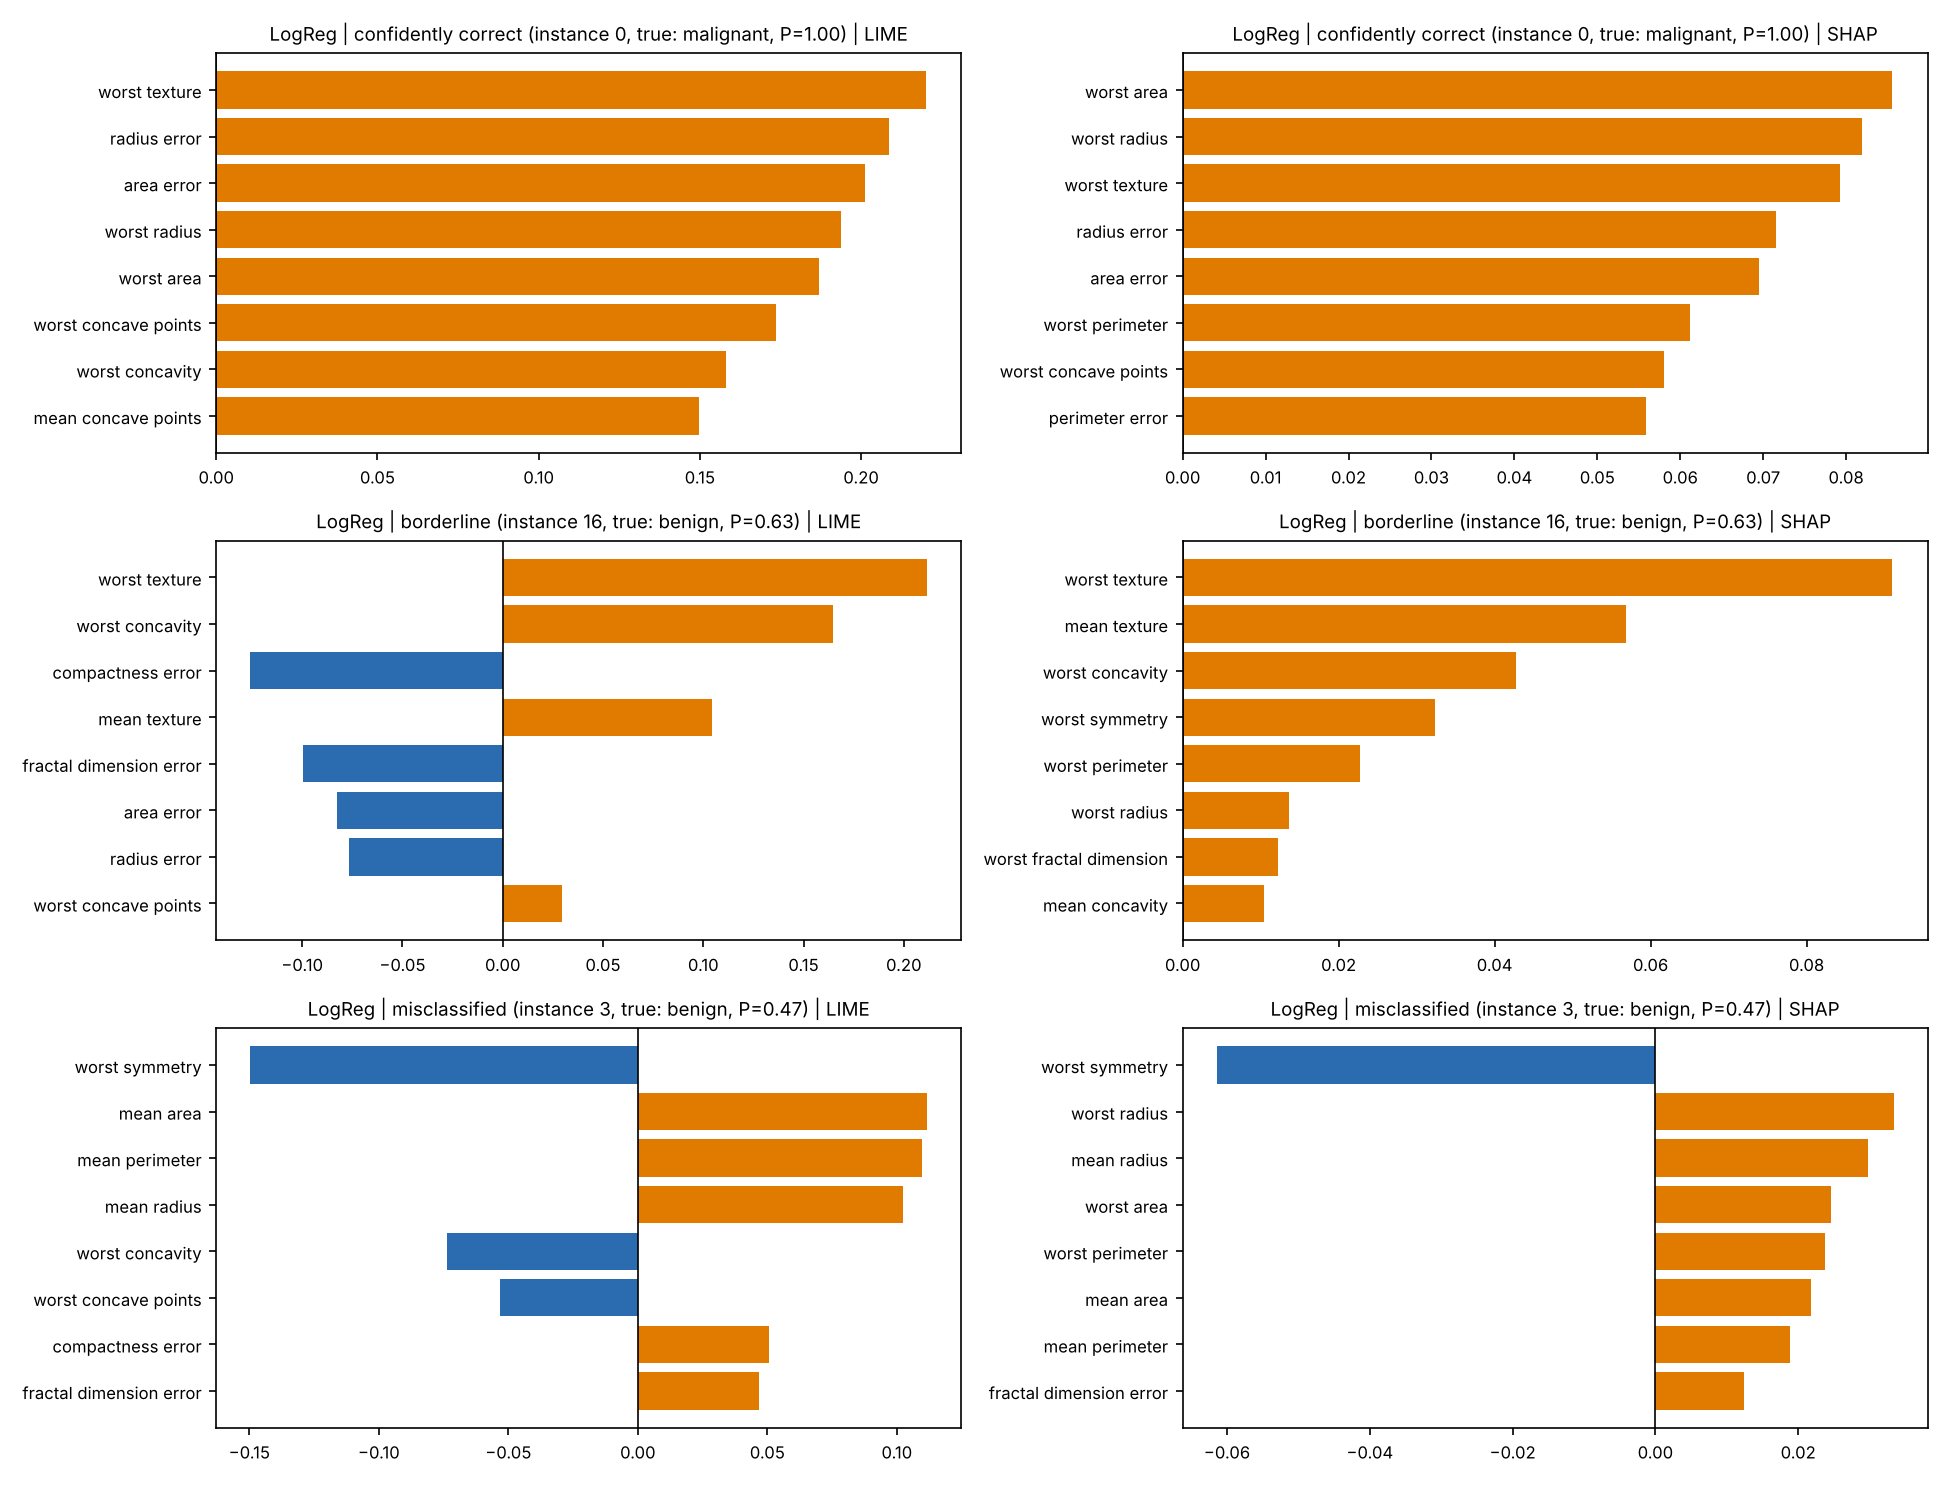
\includegraphics[width=\linewidth]{figs_en/contrib_LogReg.png}
\caption{Tương tự Hình~\ref{fig:rf} nhưng cho Logistic Regression. Ở mẫu 3, Logistic Regression dự đoán đúng ($P = 0{,}466$). Nguồn: thực nghiệm của nhóm (\coderepo).}\label{fig:lr}
\end{minipage}
\end{figure}

\subsection{LIME so với SHAP}
\label{sec:compare}
\emph{Overlap@5} là số đặc trưng xuất hiện trong cả tập top-5 của LIME và của
SHAP (xếp hạng theo $|\text{đóng góp}|$), chia cho 5; giá trị chạy từ 0
(không chung đặc trưng nào) tới 1 (cùng năm đặc trưng, không kể thứ tự).
Chúng tôi báo cáo giá trị này cho lần chạy chính và cho trung bình trên mọi
cặp lần chạy LIME--SHAP. Hệ số \emph{Spearman} $\rho \in [-1, 1]$ so sánh
cách hai phương pháp xếp hạng toàn bộ 30 đặc trưng theo
$|\text{đóng góp}|$ ($-1$ là đảo ngược, 0 là không liên quan, 1 là trùng
khớp), nên khác với Overlap@5, nó dùng tới thứ tự của mọi đặc trưng. Chúng
tôi cũng ghi lại đặc trưng đứng đầu và thời gian chạy của từng phương pháp
(Bảng~\ref{tab:compare}).

\begin{table}[!htb]
\centering\footnotesize
\caption{LIME so với SHAP trên ba mẫu. Overlap@5 ghi theo dạng lần chạy chính
/ trung bình trên mọi cặp lần chạy; thời gian chạy ghi theo dạng LIME /
SHAP.}\label{tab:compare}
\setlength{\tabcolsep}{3pt}
\begin{tabular}{@{}L{1.9cm}L{2.2cm}ccL{2.3cm}L{2.3cm}c@{}}
\toprule
\textbf{Mô hình} & \textbf{Mẫu} & \textbf{Overlap@5} & \textbf{Spearman $\rho$} & \textbf{Top-1 LIME} & \textbf{Top-1 SHAP} & \textbf{Thời gian (s)}\\
\midrule
LogReg & Đúng chắc chắn & 1,0 / 0,80 & 0,74 & worst texture & worst area & 0,035 / 0,043\\
LogReg & Sát ranh giới & 0,6 / 0,67 & 0,24 & worst texture & worst texture & 0,037 / 0,035\\
LogReg & Dự đoán sai & 0,4 / 0,49 & 0,26 & worst symmetry & worst symmetry & 0,040 / 0,034\\
Random Forest & Đúng chắc chắn & 0,8 / 0,82 & 0,83 & worst concave points & worst area & 0,066 / 0,441\\
Random Forest & Sát ranh giới & 0,6 / 0,71 & 0,69 & worst concavity & worst perimeter & 0,067 / 0,484\\
Random Forest & Dự đoán sai & 0,4 / 0,44 & 0,46 & worst concave points & worst area & 0,069 / 0,390\\
\bottomrule
\end{tabular}
\end{table}

\textbf{Mức đồng thuận giảm khi mẫu càng khó.} Với cả hai mô hình, Overlap@5
giảm từ 0,8--1,0 ở mẫu đúng chắc chắn xuống còn 0,4 ở mẫu bị dự đoán sai. Khi
một đặc trưng xuất hiện trong cả hai tập top-5, hai phương pháp luôn gán cho
nó cùng một dấu (tỉ lệ đồng dấu bằng 1,0 trong cả sáu trường hợp). Như vậy
bất đồng nằm ở chỗ \emph{đặc trưng nào} được chọn, chứ không ở hướng tác động
của chúng.

\textbf{Thứ hạng lệch nhau nhiều nhất lại ở mô hình đơn giản nhất.} Hệ số
Spearman $\rho$ thấp nhất với Logistic Regression trên hai mẫu khó (0,24 và
0,26), nghĩa là thứ hạng đầy đủ khác nhau đáng kể ngay cả với một mô hình
tuyến tính, và hai tập top-5 chỉ trùng nhau một phần (0,4--0,6). Một nguyên
nhân có thể có, nhưng chúng tôi chưa kiểm chứng, là LIME mặc định rời rạc hoá
các đặc trưng liên tục.

\textbf{Thời gian chạy.} Trên Logistic Regression, hai phương pháp mất thời
gian xấp xỉ nhau (khoảng 0,04\,s). Trên Random Forest, KernelSHAP chậm hơn
LIME khoảng 6--7 lần (0,39--0,48\,s so với khoảng 0,07\,s), vì nó truy vấn mô
hình trên $2000$ liên minh $\times$ $100$ mẫu nền. Mọi số đo thời gian đều
lấy trên cùng một máy và dao động tới khoảng 20\% giữa các lần chạy của chúng
tôi.

\subsection{Một trường hợp hai lời giải thích mâu thuẫn}\label{sec:wrong}
Bây giờ chúng tôi xem xét kỹ mẫu bị dự đoán sai (chỉ số test 3), nơi Random
Forest dự đoán $P(\text{ác tính}) = 0{,}745$ dù nhãn thật là lành tính.
Bảng~\ref{tab:wrong} liệt kê top-5 đặc trưng mà mỗi phương pháp đưa ra cho dự
đoán này. Đóng góp dương đẩy dự đoán về phía ác tính, đóng góp âm đẩy về phía
lành tính.

\begin{table}[!htb]
\centering\small
\caption{Top-5 đặc trưng của LIME và SHAP cho mẫu bị dự đoán sai (Random
Forest, chỉ số test 3). Đặc trưng xuất hiện ở cả hai phương pháp được in
đậm.}\label{tab:wrong}
\begin{tabularx}{\textwidth}{L{1.9cm}XX}
\toprule
\textbf{Phương pháp} & \textbf{Top-5 theo $|\text{đóng góp}|$} & \textbf{Dấu}\\
\midrule
LIME & worst concave points, \textbf{mean area}, \textbf{mean radius}, mean perimeter, worst concavity & worst concave points và worst concavity mang dấu âm; các đặc trưng còn lại dương\\
SHAP & worst area, worst perimeter, worst radius, \textbf{mean area}, \textbf{mean radius} & Tất cả đều dương\\
\bottomrule
\end{tabularx}
\end{table}

Hai phương pháp chỉ chia sẻ hai đặc trưng (mean area và mean radius), nên
Overlap@5 bằng 0,4, và chúng kể hai câu chuyện khác nhau về cùng một dự đoán.
SHAP quy gần như toàn bộ dự đoán cho các đặc trưng kích thước, tất cả đều đẩy
về phía ác tính. LIME cho một bức tranh lẫn lộn: đặc trưng quan trọng nhất
của nó, worst concave points, lại đẩy về phía lành tính, trong khi vài đặc
trưng kích thước đẩy về phía ác tính.

Không có chân lý nền nào cho ta biết lời giải thích nào mới đúng. Một cách
hiểu là hai phương pháp trả lời hai câu hỏi khác nhau: LIME hỏi khoảng giá
trị nào có ý nghĩa quanh mẫu này, còn SHAP đo phần đóng góp so với dự đoán
trung bình trên dữ liệu nền. Dù theo cách nào, hai phương pháp được dùng rộng
rãi lại mâu thuẫn nhau ngay trên một dự đoán sai, đúng chỗ mà người dùng cần
dựa vào lời giải thích, nên các lời giải thích phải được kiểm tra về độ trung
thực (Mục~\ref{sec:proc}).

\subsection{Độ ổn định}
\label{sec:stability}
Một lời giải thích được coi là ổn định nếu chạy lại phương pháp với những lựa
chọn ngẫu nhiên khác vẫn cho kết quả tương tự. Với LIME, chúng tôi thay đổi
seed ngẫu nhiên (20 lần chạy); với SHAP, chúng tôi thay đổi tập nền (5 lần
chạy). Chúng tôi dùng hai thước đo. \emph{Độ tương tự Jaccard} của hai tập
top-5 $A$ và $B$ là $|A \cap B| / |A \cup B|$, và chúng tôi báo cáo giá trị
trung bình trên mọi cặp lần chạy; nó bằng 1 khi mọi lần chạy đều chọn đúng
năm đặc trưng giống nhau. Lưu ý Jaccard khắt khe hơn Overlap@5: hai tập chung
nhau bốn trong năm đặc trưng có Jaccard $4/6 \approx 0{,}67$ nhưng Overlap@5
$= 0{,}8$. \emph{Top-1 chiếm ưu thế} là tỉ lệ các lần chạy mà đặc trưng đứng
đầu chính là đặc trưng được xếp thứ nhất nhiều lần nhất; nó bằng 1 khi mọi
lần chạy đều thống nhất về đặc trưng đứng đầu.
Bảng~\ref{tab:stability} trình bày kết quả.

\begin{table}[!htb]
\centering\small
\caption{Độ ổn định của top-5 đặc trưng (LIME: 20 seed; SHAP: 5 tập nền).}\label{tab:stability}
\setlength{\tabcolsep}{4pt}
\begin{tabular}{llcccc}
\toprule
\textbf{Mô hình} & \textbf{Mẫu} & \textbf{Jaccard LIME} & \textbf{Top-1 LIME} & \textbf{Jaccard SHAP} & \textbf{Top-1 SHAP}\\
\midrule
LogReg & Đúng chắc chắn & 0,78 & 0,95 & 0,68 & 0,40\\
LogReg & Sát ranh giới & 0,84 & 1,00 & 0,73 & 1,00\\
LogReg & Dự đoán sai & 0,85 & 1,00 & 0,53 & 1,00\\
Random Forest & Đúng chắc chắn & 0,94 & 0,60 & 1,00 & 1,00\\
Random Forest & Sát ranh giới & 0,72 & 0,80 & 0,73 & 1,00\\
Random Forest & Dự đoán sai & 0,74 & 1,00 & 1,00 & 1,00\\
\bottomrule
\end{tabular}
\end{table}

\textbf{Không phương pháp nào ổn định hơn một cách nhất quán.} Jaccard trung
bình chạy từ 0,72 đến 0,94 với LIME và từ 0,53 đến 1,00 với SHAP: SHAP hoàn
toàn ổn định trên hai mẫu của RF, nhưng cũng chính nó giữ giá trị thấp nhất
bảng (LR, mẫu bị dự đoán sai).

\textbf{Đặc trưng đứng đầu có thể thay đổi ngay cả trên mẫu dễ.} Top-1 chiếm
ưu thế thấp ở hai ô: 0,60 với LIME trên Random Forest và 0,40 với SHAP trên
Logistic Regression, cả hai đều ở mẫu đúng chắc chắn. Một cách lý giải mà
chúng tôi chưa kiểm chứng là khi $P$ gần bằng 1, nhiều đặc trưng đóng góp
những lượng xấp xỉ nhau, nên chỉ cần thay đổi nhỏ là đủ để hoán đổi vị trí
dẫn đầu.

\textbf{Một ví dụ bất ổn.} Hình~\ref{fig:unstable} cho thấy mỗi đặc trưng lọt
vào top-5 với tần suất bao nhiêu, trên Random Forest ở mẫu sát ranh giới. Cả
hai phương pháp hầu như luôn chọn worst concavity, worst texture và worst
perimeter; chúng khác nhau ở vị trí 4 và 5. LIME chọn mean texture trong
100\% số lần chạy và area error trong 45\%, trong khi SHAP chọn mean concave
points trong 100\% số lần chạy (LIME chỉ 10\%) và mean texture chỉ trong
40\%. Đặc trưng đứng đầu của LIME cũng thay đổi giữa các seed: seed 0 xếp
worst concavity thứ nhất, còn các seed 1--5 xếp worst texture thứ nhất.

\begin{figure}[!htb]
\centering
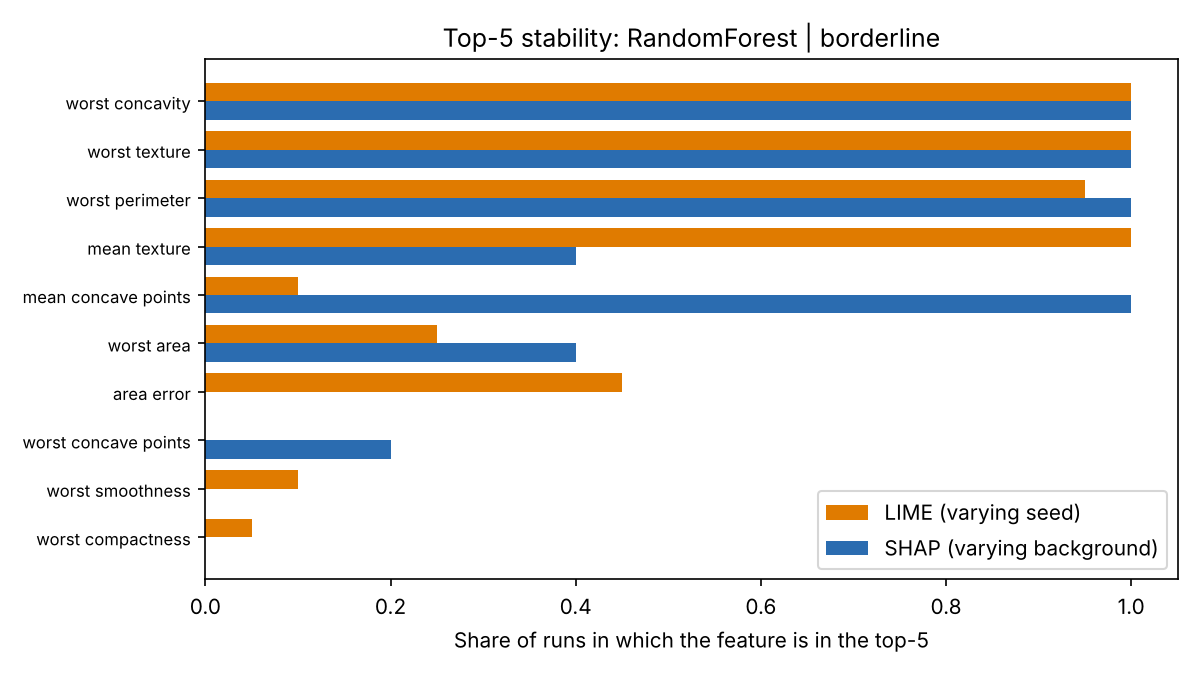
\includegraphics[width=0.6\textwidth]{figs_en/unstable_example.png}
\caption{Tỉ lệ các lần chạy mà mỗi đặc trưng xuất hiện trong top-5, Random
Forest, mẫu sát ranh giới (LIME: 20 seed; SHAP: 5 tập nền). Nhãn trên hình là
tiếng Anh. Nguồn: thực nghiệm của nhóm (\coderepo).}\label{fig:unstable}
\end{figure}

\textbf{Tinh chỉnh tham số không loại bỏ được sự bất ổn.} Thay đổi kích thước
tập nền của SHAP và độ rộng kernel của LIME trên mẫu này
(Phụ lục~\ref{app:sensitivity}) không bao giờ nâng được độ tương tự Jaccard
lên trên 0,73.

\subsection{Kiểm tra độ trung thực bằng deletion test}
\label{sec:deletion}
Một lời giải thích là trung thực nếu những đặc trưng nó đánh dấu là quan
trọng thực sự chi phối dự đoán của mô hình. Chúng tôi kiểm tra điều này bằng
cách xoá dần các đặc trưng và quan sát dự đoán thay đổi ra sao. Với mỗi mẫu
trong 20 mẫu kiểm thử được chọn ngẫu nhiên, chúng tôi lấy những đặc trưng mà
lời giải thích cho là ủng hộ lớp được dự đoán mạnh nhất, lần lượt xoá từng
đặc trưng (tối đa 10) bằng cách thay nó bằng giá trị trung bình trên tập huấn
luyện, rồi ghi lại xác suất của lớp được dự đoán sau mỗi lần xoá. Nếu lời
giải thích là trung thực, xác suất này phải giảm nhanh. Làm mốc so sánh,
chúng tôi xoá các đặc trưng theo thứ tự ngẫu nhiên và lấy trung bình trên 10
hoán vị ngẫu nhiên. Hình~\ref{fig:del} trình bày các đường cong trung bình.

\begin{figure}[!htb]
\centering\small
\pgfplotsset{delplot/.style={width=0.43\textwidth,height=4.6cm,xlabel={Số đặc trưng bị xoá},xmin=0,xmax=10,ymin=0.5,ymax=1.0,
  xtick={0,2,4,6,8,10},grid=major,grid style={gray!25},tick label style={font=\scriptsize},label style={font=\footnotesize},
  title style={font=\footnotesize\bfseries},legend style={font=\scriptsize,at={(0.03,0.03)},anchor=south west,draw=none,fill=white,fill opacity=0.8},
  every axis plot/.append style={thick}}}
\begin{tikzpicture}
\begin{axis}[delplot,title={Random Forest},ylabel={Xác suất của lớp dự đoán}]
\addplot[color=orange!85!black,mark=*,mark size=1.5pt] coordinates {(0,0.923)(1,0.827)(2,0.777)(3,0.734)(4,0.717)(5,0.698)(6,0.674)(7,0.644)(8,0.629)(9,0.610)(10,0.605)};
\addplot[color=blue!70!black,mark=square*,mark size=1.5pt] coordinates {(0,0.923)(1,0.846)(2,0.776)(3,0.732)(4,0.701)(5,0.679)(6,0.651)(7,0.625)(8,0.602)(9,0.583)(10,0.563)};
\addplot[color=gray,dashed] coordinates {(0,0.923)(1,0.918)(2,0.909)(3,0.899)(4,0.888)(5,0.877)(6,0.869)(7,0.857)(8,0.847)(9,0.839)(10,0.830)};
\legend{LIME,SHAP,Ngẫu nhiên}
\end{axis}
\end{tikzpicture}\hfill
\begin{tikzpicture}
\begin{axis}[delplot,title={Logistic Regression}]
\addplot[color=orange!85!black,mark=*,mark size=1.5pt] coordinates {(0,0.941)(1,0.914)(2,0.892)(3,0.865)(4,0.836)(5,0.802)(6,0.753)(7,0.716)(8,0.675)(9,0.634)(10,0.579)};
\addplot[color=blue!70!black,mark=square*,mark size=1.5pt] coordinates {(0,0.941)(1,0.915)(2,0.889)(3,0.865)(4,0.836)(5,0.805)(6,0.774)(7,0.731)(8,0.693)(9,0.639)(10,0.584)};
\addplot[color=gray,dashed] coordinates {(0,0.941)(1,0.940)(2,0.937)(3,0.938)(4,0.937)(5,0.934)(6,0.933)(7,0.929)(8,0.927)(9,0.925)(10,0.923)};
\legend{LIME,SHAP,Ngẫu nhiên}
\end{axis}
\end{tikzpicture}
\caption{Deletion test: xác suất trung bình của lớp được dự đoán khi lần lượt
xoá các đặc trưng xếp hạng cao nhất (20 mẫu kiểm thử, một seed). Giảm càng
nhanh thì lời giải thích càng trung thực. Nguồn: tệp
\code{results/deletion\_curves.csv} của nhóm (\coderepo).}\label{fig:del}
\end{figure}

Cả LIME và SHAP đều kéo xác suất xuống nhanh hơn hẳn so với xoá ngẫu nhiên.
Sau 5 lần xoá, Random Forest giảm từ 0,923 xuống 0,698 (LIME) và 0,679
(SHAP), nhưng chỉ xuống 0,877 khi xoá ngẫu nhiên; Logistic Regression giảm từ
0,941 xuống 0,802, 0,805 và 0,934. LIME và SHAP chênh nhau nhiều nhất 0,02 ở
mốc 5 đặc trưng và 0,04 ở mốc 10 (RF: 0,605 so với 0,563), mức chênh này,
với chỉ một seed, 20 mẫu và không có khoảng tin cậy, là chưa đủ để xếp hạng
hai phương pháp. Cảnh báo: thay bằng giá trị trung bình có thể tạo ra những
mẫu nằm ngoài phân phối, và với các đặc trưng tương quan mạnh thì xoá một đặc
trưng không xoá được thông tin của nó.

\subsection{Độ quan trọng của đặc trưng không phải là hiệu ứng nhân quả}
\label{sec:causal}
LIME và SHAP mô tả cách \emph{mô hình} sử dụng các đặc trưng của nó, chứ
không mô tả những đặc trưng ấy ảnh hưởng ra sao tới \emph{bệnh}: phần đóng
góp lớn nghĩa là mô hình dựa nhiều vào một đặc trưng, không có nghĩa đặc
trưng đó gây ra ác tính. Có bốn lý do, đều thấy được trong thực nghiệm của
chúng tôi, cho thấy vì sao không nên lẫn lộn hai điều này.

\begin{itemize}
  \item \textbf{Đặc trưng tương quan.} Worst radius, perimeter và area cùng
        tăng với nhau và đều nằm gần đầu các biểu đồ; việc chia công trạng
        giữa chúng phụ thuộc vào mô hình và dữ liệu nền, chứ không phụ thuộc
        vào đặc trưng nào mới là nguyên nhân thật sự.
  \item \textbf{Mẫu phi thực tế.} Cả LIME và KernelSHAP đều thay đổi từng đặc
        trưng độc lập với các đặc trưng khác; với KernelSHAP đây chính là giả
        định độc lập đặc trưng được mô tả ở Mục~\ref{sec:shap}. Điều này tạo
        ra những tổ hợp không bao giờ xuất hiện ở khối u thật, chẳng hạn diện
        tích lớn đi kèm bán kính nhỏ, nên mô hình bị truy vấn ở những vùng nó
        chưa từng thấy dữ liệu.
  \item \textbf{Lời giải thích cũng phản ánh sai lầm của mô hình.} Ở mẫu bị
        dự đoán sai (Mục~\ref{sec:wrong}), các đặc trưng kích thước giải
        thích vì sao mô hình sai, chứ không chứng minh khối u là ác tính.
  \item \textbf{Thay một giá trị không phải là một can thiệp thật.} Đó chỉ là
        một phép tính trên mô hình; muốn biết điều gì xảy ra nếu kích thước
        khối u thực sự thay đổi thì cần những giả định nhân quả mà cả hai
        phương pháp đều không kiểm chứng.
\end{itemize}
Vì vậy, kết luận nên được diễn đạt là ``mô hình dựa vào $X$'', chứ không phải
``$X$ gây ra $Y$''.

\subsection{Quy trình đánh giá độ trung thực (đề xuất)}\label{sec:proc}
Vì LIME và SHAP có thể mâu thuẫn nhau và thay đổi giữa các lần chạy, chúng
tôi đề xuất quy trình năm bước dưới đây, được tổ chức (theo tinh thần, không
theo công thức chính xác) quanh các tiêu chí của Mersha và cộng
sự~\cite{mersha}. Mỗi bước nêu rõ tiêu chí tương ứng và việc chúng tôi đã
thực hiện hay chưa.

\begin{enumerate}
  \item \textbf{Kiểm tra trên một bài toán đã biết đáp án} (độ trung thực).
        Với mô hình tuyến tính, lời giải thích phải khớp với
        $w_j (x_j - \mu_j)$. \emph{Trạng thái:} đã làm trên ví dụ tính tay
        (Mục~\ref{sec:shaphand}), chưa làm trên mô hình LR của thực nghiệm.
  \item \textbf{Độ khớp cục bộ} (độ trung thực). LIME: $R^2$ có trọng số của
        mô hình thay thế quanh $x$; SHAP: $\varphi_0 + \sum_j \varphi_j = f(x)$.
        \emph{Trạng thái:} đã kiểm tra với SHAP (Mục~\ref{sec:charts}); chưa
        tính $R^2$ của LIME.
  \item \textbf{Deletion và insertion so với thứ tự ngẫu nhiên} (độ trung
        thực, tính đầy đủ). \emph{Trạng thái:} đã làm deletion
        (Mục~\ref{sec:deletion}); chưa làm insertion.
  \item \textbf{Độ ổn định} (tính nhất quán). Jaccard top-$k$ và phương sai
        của nó qua nhiều seed và nhiều tập nền. \emph{Trạng thái:} đã làm
        (Mục~\ref{sec:stability}, Phụ lục~\ref{app:sensitivity}).
  \item \textbf{Tính bền vững.} Mức thay đổi của lời giải thích khi đầu vào bị
        nhiễu nhẹ hoặc khi đổi sang mô hình có độ chính xác tương đương.
        \emph{Trạng thái:} chưa làm.
\end{enumerate}

Hiệu quả được đo bằng thời gian chạy (Mục~\ref{sec:compare}). Một lời giải
thích chỉ nên được coi là đáng tin khi nó vượt qua đồng thời nhiều bước kiểm
tra trong số này; vượt qua một bước đơn lẻ là chưa đủ.

%---------------------------------------------------------------------
\section{Kết luận}
Câu trả lời của chúng tôi cho câu hỏi dẫn dắt là không: một dự đoán có độ
chính xác cao không nhất thiết đi kèm một lời giải thích đáng tin cậy. Dù hai
mô hình đạt độ chính xác 98,2\% và 95,6\% trên tập kiểm thử, LIME và SHAP chỉ
chia sẻ hai trong năm đặc trưng quan trọng nhất ở mẫu bị dự đoán sai
(Overlap@5 $= 0{,}4$). Tập top-5 của mỗi phương pháp cũng thay đổi giữa các
lần chạy, với độ tương tự Jaccard trung bình thấp tới 0,53 với SHAP và 0,72
với LIME. Trong deletion test, cả hai phương pháp đều tìm ra đặc trưng có ảnh
hưởng tốt hơn hẳn thứ tự ngẫu nhiên, nhưng không phương pháp nào được chứng
minh là trung thực hơn, và không phương pháp nào cho biết quan hệ nhân quả.

\textbf{Điều kiện sử dụng.} Một lời giải thích mô tả hành vi của mô hình,
hoặc quanh một mẫu (LIME) hoặc so với một giá trị nền (SHAP). Người dùng nên
ghi rõ seed, dữ liệu nền và độ rộng kernel, lặp lại việc giải thích và báo
cáo độ ổn định của nó, đồng thời áp dụng các bước kiểm tra ở
Mục~\ref{sec:proc}, nhất là với những mẫu sát ranh giới và những mẫu bị dự
đoán sai.

\textbf{Hạn chế và hướng phát triển.} Với một bộ dữ liệu, ba mẫu, hai mô hình
và không có khoảng tin cậy, các kết luận ở đây mang tính minh hoạ
(Phụ lục~\ref{app:limits}). Các bước tiếp theo là insertion test, tính $R^2$
của LIME, dùng TreeSHAP, chuyển sang thang log-odds, thử thêm nhiều bộ dữ
liệu và tăng số lần lặp.

%---------------------------------------------------------------------
\begin{thebibliography}{9}
\bibitem{ribeiro} Ribeiro, M. T., Singh, S., \& Guestrin, C. (2016). ``Why Should I Trust You?'': Explaining the Predictions of Any Classifier. \emph{KDD 2016}, 1135--1144. \href{https://doi.org/10.1145/2939672.2939778}{DOI}.
\bibitem{mersha} Mersha, M., Lam, K., Wood, J., AlShami, A., \& Kalita, J. (2024). Explainable artificial intelligence: A survey of needs, techniques, applications, and future direction. \emph{Neurocomputing}, 599, 128111. \href{https://doi.org/10.1016/j.neucom.2024.128111}{DOI} (chúng tôi đọc bản arXiv 2409.00265v2).
\bibitem{lundberg} Lundberg, S. M., \& Lee, S.-I. (2017). A Unified Approach to Interpreting Model Predictions. \emph{NeurIPS 2017}. \href{https://proceedings.neurips.cc/paper_files/paper/2017/hash/8a20a8621978632d76c43dfd28b67767-Abstract.html}{Trang bài báo}.
\bibitem{street} Street, W. N., Wolberg, W. H., \& Mangasarian, O. L. (1993). Nuclear feature extraction for breast tumor diagnosis. \emph{IS\&T/SPIE 1993 International Symposium on Electronic Imaging: Science and Technology}, vol.\ 1905, 861--870. \href{https://api.semanticscholar.org/CorpusID:14922543}{Trang bài báo}.
\end{thebibliography}

\section*{Dữ liệu, công cụ và nguồn số liệu}
\begin{itemize}
  \item \textbf{Dữ liệu.} Breast Cancer Wisconsin (Diagnostic) \cite{street},
        nạp bằng\\ \code{sklearn.datasets.load\_breast\_cancer}.
  \item \textbf{Phần mềm.} Python với các thư viện scikit-learn, \code{lime}
        và \code{shap}.
  \item \textbf{Nguồn số liệu.} Toàn bộ hình, bảng, số liệu và cả hai ví dụ
        tính tay đều do nhóm tạo ra bằng notebook
        \code{S04\_LIME\_SHAP\_}\allowbreak\code{experiments.ipynb}; không có
        số liệu nào lấy từ các bài báo được trích dẫn.
  \item \textbf{Việc sử dụng công cụ AI.} Claude (Anthropic) được dùng để hỗ
        trợ giải thích khái niệm, viết mã thực nghiệm, soạn và chỉnh sửa báo
        cáo này.
  \item \textbf{Kiểm chứng nội dung có hỗ trợ của AI.} Chúng tôi đã đối chiếu
        mọi phát biểu về LIME và SHAP với các bài báo gốc
        \cite{ribeiro}\cite{lundberg} và bài khảo sát \cite{mersha}; chạy lại
        notebook và so từng con số trong bảng và trong phần nội dung với các
        tệp CSV trong \code{results/}; và tính lại độc lập cả hai ví dụ tính
        tay (bằng tay và bằng một đoạn mã NumPy ngắn).
  \item \textbf{Kho mã nguồn.} Notebook và toàn bộ kết quả thực nghiệm của
        chúng tôi có tại
        \url{https://github.com/khoiLearnsToCode/CS420_AI_LIME_SHAP}.
  \item \textbf{Về bản dịch này.} Đây là bản tiếng Việt của \code{Report.tex}.
        Mọi số liệu, bảng, công thức và kết luận giữ nguyên như bản tiếng
        Anh. Tên đặc trưng (\code{worst area}, \code{mean radius}, \dots) giữ
        nguyên tiếng Anh để khớp với tên cột trong dữ liệu, với mã nguồn và
        với nhãn trên các hình trong \code{figs\_en/}.
\end{itemize}

%---------------------------------------------------------------------
\appendix
\section{Thiết lập thực nghiệm đầy đủ}\label{app:setup}

\begin{table}[!htb]
\centering\small
\caption{Thiết lập thực nghiệm.}\label{tab:setup}
\begin{tabularx}{\textwidth}{L{2.4cm}XL{3.8cm}}
\toprule
\textbf{Thành phần} & \textbf{Lựa chọn} & \textbf{Lý do}\\
\midrule
Dữ liệu & Breast Cancer Wisconsin \cite{street}, nạp từ scikit-learn: 569 mẫu, 30 đặc trưng, lớp 0 = ác tính, lớp 1 = lành tính; chia phân tầng 80/20 với \code{random\_state = 42} (455 huấn luyện, 114 kiểm thử) & Công khai, nhị phân và dễ tiếp cận\\
Mô hình & Logistic Regression (có chuẩn hoá) và Random Forest 200 cây; độ chính xác kiểm thử 98,2\% và 95,6\% & Một mô hình tuyến tính làm mốc tham chiếu và một mô hình kém minh bạch hơn để bộc lộ sự bất ổn\\
Không gian giải thích & Xác suất $P(\text{ác tính})$ & LIME giải thích xác suất dự đoán \cite{ribeiro}, nên lựa chọn này giúp hai phương pháp so sánh trực tiếp được với nhau. Hệ quả là các giá trị $\varphi$ cộng lại trên thang xác suất, không phải trên thang log-odds\\
SHAP & KernelSHAP \cite{lundberg} với 100 mẫu nền lấy từ tập huấn luyện và 2000 liên minh được lấy mẫu & Dùng cùng một công cụ độc lập mô hình cho cả hai mô hình, nên thời gian chạy so sánh được\\
LIME & 5000 mẫu nhiễu, độ rộng kernel mặc định $0{,}75\sqrt{d} \approx 4{,}11$, rời rạc hoá mặc định & Cấu hình chuẩn của thư viện\\
Ba mẫu & Một quy tắc cố định áp dụng trên RF: dự đoán đúng có độ tin cậy cao nhất (chỉ số 0), dự đoán có $|P - 0{,}5|$ nhỏ nhất (chỉ số 16) và mẫu bị dự đoán sai đầu tiên (chỉ số 3) & Ngăn việc chọn những ví dụ có lợi\\
Số lần chạy & LIME: 20 seed; SHAP: 5 tập nền (seed 0--4); top-$k$ với $k = 5$ & Dung hoà giữa việc đo được độ ổn định và giữ thời gian chạy ở mức thấp\\
Deletion test & 20 mẫu kiểm thử ngẫu nhiên (seed cố định); xoá tối đa 10 đặc trưng bằng cách thay bằng giá trị trung bình trên tập huấn luyện & Kiểm tra độ trung thực\\
\bottomrule
\end{tabularx}
\end{table}

\section{Độ nhạy theo kích thước tập nền và độ rộng kernel}\label{app:sensitivity}
Mục~\ref{sec:stability} đã cho thấy lời giải thích thay đổi giữa các lần
chạy. Ở đây chúng tôi kiểm tra xem sự bất ổn này có giảm được bằng cách thay
đổi tham số chính của mỗi phương pháp hay không: kích thước tập nền với SHAP
và độ rộng kernel với LIME. Chúng tôi dùng Random Forest trên mẫu sát ranh
giới, trường hợp mà LIME kém ổn định nhất (Jaccard 0,72) và SHAP cũng không
hoàn toàn ổn định (0,73). Với mỗi kích thước tập nền, chúng tôi chạy SHAP
trên 5 tập nền; với mỗi độ rộng kernel, chúng tôi chạy LIME với 10 seed. Vì ở
đây LIME dùng ít seed hơn so với 20 seed ở Mục~\ref{sec:stability}, các giá
trị Jaccard của nó không so sánh trực tiếp được với
Bảng~\ref{tab:stability}. Bảng~\ref{tab:sensitivity} trình bày kết quả.

\begin{table}[!htb]
\centering\small
\caption{Độ nhạy theo tham số (Random Forest, mẫu sát ranh giới).}\label{tab:sensitivity}
\begin{tabular}{llcc}
\toprule
\textbf{Phương pháp} & \textbf{Tham số} & \textbf{Jaccard top-5} & \textbf{Top-1 chiếm ưu thế}\\
\midrule
SHAP & tập nền = 10 & 0,63 & 0,8\\
SHAP & tập nền = 50 & 0,73 & 1,0\\
SHAP & tập nền = 100 (mặc định) & 0,73 & 1,0\\
LIME & độ rộng kernel = 1,00 & 0,65 & 0,7\\
LIME & độ rộng kernel = 2,00 & 0,68 & 0,9\\
LIME & độ rộng kernel = 4,11 (mặc định) & 0,68 & 0,9\\
LIME & độ rộng kernel = 8,00 & 0,68 & 0,9\\
\bottomrule
\end{tabular}
\end{table}

Với SHAP, tập nền chỉ gồm 10 mẫu làm giảm độ ổn định (Jaccard 0,63), nhưng
tăng lên quá 50 thì không cải thiện thêm (0,73). Với LIME, độ rộng kernel nhỏ
bằng 1,0 kém ổn định hơn một chút (0,65), còn mọi độ rộng từ 2,0 trở lên đều
cho cùng kết quả (0,68). Ngay cả thiết lập tốt nhất cũng còn cách xa 1, nên
việc tinh chỉnh các tham số này không loại bỏ được sự bất ổn trên mẫu đang
xét.

\section{Hạn chế}\label{app:limits}
\begin{itemize}
  \item Chỉ một bộ dữ liệu, ba mẫu và hai mô hình; kết quả có thể không tổng quát hoá được.
  \item 20 seed (LIME) và 5 tập nền (SHAP) là ít, và không có khoảng tin cậy.
  \item Deletion test chỉ dùng một seed và 20 mẫu, và việc thay bằng giá trị trung bình có thể tạo ra mẫu nằm ngoài phân phối.
  \item Thời gian chạy đo trên một máy và chỉ với KernelSHAP; dùng TreeSHAP cho Random Forest sẽ nhanh hơn nhiều (chưa đo).
  \item Lời giải thích nằm trên thang xác suất; trên thang log-odds kết quả có thể khác (chưa kiểm chứng).
  \item LIME rời rạc hoá các đặc trưng, nên chỉ có thể so sánh thứ hạng và dấu với SHAP, không so sánh được độ lớn tuyệt đối.
  \item Không có chân lý nền cho các lời giải thích của Random Forest, nên chúng tôi không thể khẳng định phương pháp nào là ``đúng''.
\end{itemize}

\end{document}
